\documentclass[a4paper,12pt]{report}
\usepackage{graphicx}
\usepackage{titlesec}
\titleformat{\chapter}{}{}{0em}{\bf\LARGE}
\usepackage[utf8]{inputenc}
% Title Page
\title{Middle East Technical University\\Department of Physics\\PHYS222 Optics and Waves Laboratory\\\textbf{Experiment OW-4 Polarization\\Laboratory Report}}

\author{Oğuzhan ÖZCAN\\1852334\\\\Partner: İnci SAİM\\\\Teaching Assistant: Hikmet ÖZŞAHİN}


\begin{document}
\maketitle
\tableofcontents
\listoffigures

\chapter{Theory}
The meaning of the polarization is that the ability to manipulate light. The simplest method of polarizing a light is discovered by Malus in 1808. His method consist of a polished surface and a beam of white light at a certain angle. When beam of white light incident with plane, reflection would be plane-polarized $[1]$.\\\\
As we know light is a transverse wave like electromagnetic waves. All waves have electric and magnetic field and these fields are perpendicular to each other. When a wave lies on the x-axis, the displacement should be through the y-axis. In this sende, we consider that wave is along the xy-plane. For instance, if a wave has only y-displacement then we say that this wave is linearly polarized in the y-direction $[2]$. As we mentioned before waves have two components: electric field \textbf{E} and magnetic field \textbf{B}. These components can be described as mathematically
\begin{center}
	$\vec{E}(x,t)=\hat{j}E_{0}\cos(kx-\omega t)$\\$\vec{B}(x,t)=\hat{k}B_{0}\cos(kx-\omega t)$
\end{center}
The electric field and magnetic field of an ideal monochromatic light must oscillate at a definite frequency so x-component and y-component can oscillate independently. That means these components may be either in phase or out of phase.\\\\
If we go through the terminology there are three types of polarization: \textit{linear (plane) polarization, elliptical polarization and circular polarization.} These three types of polarized lights are differ from each other  according to their geometrical shapes (See Figure 1.), properties etc.\\\\
\textbf{Linear (Plane) Polarization}\\
When the electric field oscillates on a straight line, the light would be linearly polarized. In this type of polarization the orientation of the electric field is constant [3]. The two orthogonal optical disturbances can be represented as  
\begin{center}
	$\vec{E}_{x}(z,t)=-\hat{i}E_{0x}\cos(kz-\omega t)$\\$\vec{E}_{y}(z,t)=\hat{j}E_{0y}\cos(kz-\omega t+\epsilon)$
\end{center}
where $\epsilon$ is correspond to relative phase difference betweend the waves. Note that both waves are travelling in z-direction. We can simplfy the resultant optical disturbance as 
\begin{center}
	$\vec{E}(z,t)=\vec{E}_{x}(z,t)+\vec{E}_{y}(z,t)$
\end{center}
When $\epsilon$ is zero then we say that waves are in phase. Obviously a linear polarizer is a device that produces linearly produces light from unpolarized light. There are several kinds of linear polarizers. The most efficient linear polarizers are based on the principle of double refraction $[4]$. Note that the dichroism is also related to linear polarization. 
\begin{figure}[h]
\centering
\includegraphics[width=1.0\linewidth, height=0.3\textheight]{"Types of polarization"}
\caption{Types of Polarization}
\label{fig:Typesofpolarization}
\end{figure}
\\
\textbf{Circular Polarization}\\
When the electric field vectors travels around a circle then we have a light beam which is circulary polarized. In this case both waves have same amplitude
\begin{center}
	$E_{0}=E_{0x}=E_{0y}$ 
\end{center}
In this sense the relative phase difference is $\epsilon=-\pi/2+2m\pi$ where \textit{m} is equal to $m=\pm1,\pm2,\pm3,...$ Therefore the electric field equations will be  
\begin{center}
	$\vec{E}_{x}(z,t)=\hat{i}E_{0x}\cos(kz-\omega t)$\\$\vec{E}_{y}(z,t)=\hat{j}E_{0y}\sin(kz-\omega t)$
\end{center}
Thus the resulting wave will be
\begin{center}
	$\vec{E}=E_{0}[\hat{i}\cos(kz-\omega t)+\hat{j}\sin(kz-\omega t)]$
\end{center}
There are two types of circular polarized light: the right-hand circular polarized light and the left-hand circular polarized light. When we look at the electric vector if it as the light comes straight toward us and goes around in a counter-clockwise direction then we call it right-hand circular polarization and the opposite situation called as left-hand circular polarization $[5]$. The circular polarization is a well-known method to give a criterion to distinguish between prolate and oblate crystals $[6]$.\\\\
\textbf{Elliptical Polarization}\\
Both linearly polarized light and circularly polarized light may be considered as special cases of elliptically polarized light. In elliptical polarization the resultant electric field vector $\vec{E}$ rotate and change its magnitude. We can see the difference by the following equations  
\begin{center}
	$E_{x}=E_{0x}\cos(kz-\omega t)$\\$E_{y}=E_{0y}\cos(kz-\omega t+\epsilon)$
\end{center}
Previous equations shows that an elliptical polarized light is the superposition of two orthogonal and linearly polarized lights $[7]$.\\\\
\textbf{Unpolarized Light}\\
An ordinary beam of light contains a large number of electromagnetic waves. These waves emitted by atoms whose have random vibrational orientation. That means these waves locations are not certain. That is why these electric field vector $\vec{E}$ in the beam is random $[8]$. In this case we say that the beam of light is unpolarized. A beam of unpolarized light can be polarized by reflection, refraction, scattering and absorption.\\\\
\textbf{Law of Malus }\\
The Malus's law is a formula for calculating intensity of the polarized light through the analyzer with an angle of $\theta$ and this law show that the intensity of the beam is proportional to the square of the cosine of the ray angle $[9]$ 
\begin{center}
	$I=A^{2}\cos^{2}(\theta)$
\end{center}
where $A$ is a constant. In figure 1.2, relation between $A$ and intensity $I$ can be seen easily.
\newpage
\begin{figure}[h]
\centering
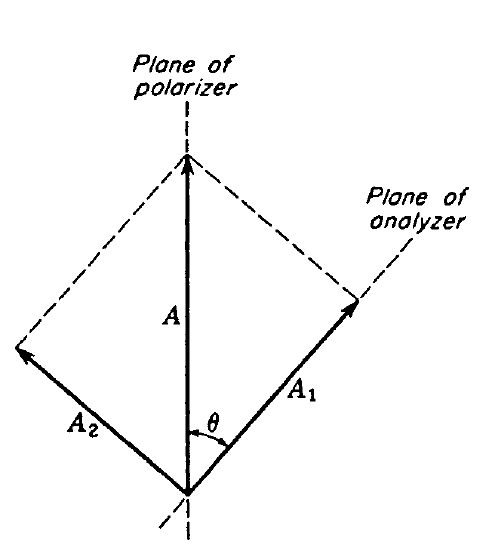
\includegraphics[width=0.4\linewidth, height=0.29\textheight]{malus}
\caption{Components of the amplitude of a plane-polarized light}
\label{fig:malus}
\end{figure}
The intensity can be calculated as 
\begin{center}
	$I=A_{1}^{2}=A^{2}\cos^{2}(\theta)=I_{0}\cos^{2}(\theta)$
\end{center}
where $I_{0}$ is correspond to intensity of the incident polarized light. The resultant Malus's law comes from polarization process. Assume that we have we are polarizing a beam of light. There is full transformation for one sense of polarization and full absorption for the orthogonal sense. Then if we write electric fields for polarizer and analyser []
\begin{center}
	$E_{p}=E_{0}\cos(kx-\omega t)[e_{x}\cos\theta+e_{y}\cos\theta]$ and\\
$E_{a}=E_{0}\cos(kx-\omega t)e_{x}\cos\theta$
\end{center}
Thus time averaged intensity will be 
\begin{center}
	$I(\theta)=[\epsilon_{0}c/2]E_{0}^{2}\cos^{2}\theta=I_{0}cos^{2}(\theta)$
\end{center}




\chapter{Data and Results}
\textbf{1. Plot a graph with measured intensities $I(\theta)$ as ordinates and the angle $\theta$ between the polarizers as abscissa. Does it appear to fit to a function of the form $I(\theta)=a+b\cos^{2}\theta$? If yes explain.}
\begin{figure}[h]
\centering
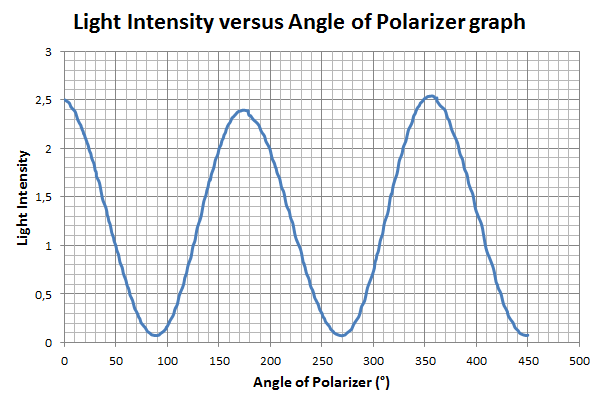
\includegraphics[width=1.05\linewidth, height=0.5\textheight]{graph}
\caption{Light Intensity versus Angle of Polarizer graph}
\label{fig:graph}
\end{figure}
\\
Our graph is fit to a function of the form $I(\theta)=a+b\cos^{2}\theta$ because the graph should be similar to cosine graph since we have a $\cos^{2}$ factor.\\
\textbf{2. Which type of polarization do you observe? (i.e. Linear, circular or elliptical polarization)}\\
We have observed linear polarization in this experiment.



\chapter{Discussion and Conclusion}
\textbf{1.What are the possible errors in the experiment?}\\
The most possible error was angular speed of the polarizer. We were turning polarizer manually and speed was not constant. We did not consider distances between laser beam, polarizer and analyzer. This may cause some errors. Since we were working with electronical tools and as we know there is no electronic devices that can measure 100\% correctly so this is another possible error.\\\\
\textbf{2.What kind of approximation did you take into consideration while you were obtaining the physical quantities and how do they affect your results?}\\
The only approximation was turning the polarizer. We had to be at constant speed but of course we should have some acceleration and deceleration during the process.\\\\
\textbf{3.What discrepancies did you encounter between the calculated quantities and theoretical or literature values?}\\
Apperantly there is no certain discrepancies about our experiment. Because our graph is almost as correct as theoretical one. When we look at the graph we can see that in $2\pi$ or $360^{\circ}$, the light intensity almost same with starting value. To see the experiment's success I would like to present an experimental data in Figure 3.1, from \textit{Laser Teaching Center-Department of Physics and Astronomy, Stony Brook University, USA.}
\begin{figure}[h]
\centering
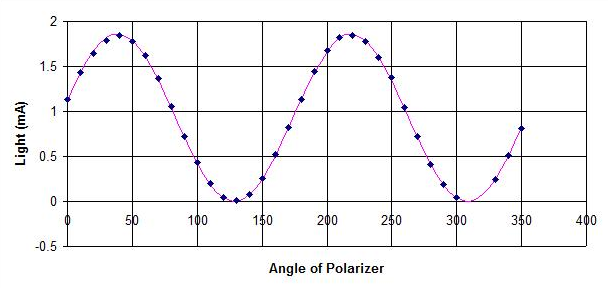
\includegraphics[width=1.0\linewidth, height=0.30\textheight]{stoony}
\caption{Theoretical and Experimental Values for Malus's Law}
\label{fig:stoony}
\end{figure}
As seen our graph and represented graph are so similar.\\\\  
\textbf{4.What is your overall conclusion?}\\
To sum up, we can say that experiment was succesful. We have seen the linear polarization during the experiment. Experimental and theoretical values are verify each other. I think that \textit{a} is the constant of imperfection of the polarizer in blocking light when it is perpendicular and \textit{b} is the maximized transmittance. Alternatively we can say that $a=k_{2}$ and $b=k_{1}$. If $a=0$, then $b=1$. By using this relation we can get the formula of law of Malus as 
\begin{center}
	$I_{out}=\frac{1}{2}I_{in}\cos^{2}(\theta)$  
\end{center}
\chapter{Applications}
\textbf{Polarizing Microscopes}\\\\
A polarizing microscope is a special microscope that uses
polarized light for investigating the optical properties of
specimens. Although originally called a mineral microscope
because of its applications in petrographic and
mineralogical research, in recent years it has now come
to be used in such diverse fields as biology, medicine,
polymer chemistry, liquid crystals, magnetic memory,
and state-of-the-art materials. There are two types of
polarizing microscopes: transmitted light models and
incident light models. Figure 4.1 shows the basic construction
of a transmitted light polarizing microscope.
\begin{figure}[h]
	\centering
	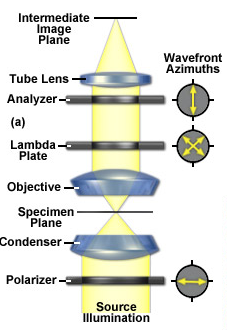
\includegraphics[width=0.30\linewidth, height=0.28\textheight]{app2}
	\caption{Polarized Light Microscope Optical Pathways}
	\label{fig:app2}
\end{figure}
A polarizing microscope has a new construction
with the following added units: a polarizing
condenser that includes a polarizer, a rotating
stage that allows the position of the specimen to
be set, a strain-free objective for polarized light, a
centerable revolving nosepi ece that allows optical
axis adjustment for the objective, an analyzer,
a Bertrand lens for observing the pupil of the
objective, a test plate, a compensator, and an
eyepiece with crosshair $[11]$. 
\chapter{References}
\textbf{1}	Jenkins, F., & White, H. (2001). \textit{Fundamentals of Optics} (4th ed., p. 498). New York: McGraw-Hill.\\
\textbf{2} Young, H. (2012). \textit{University Physics with Modern Physics: Sears and Zemansky's} (13th ed., p. 1093). Boston: Pearson education.\\
\textbf{3} Hecht, E. (2002). \textit{Optics} (4th ed., p. 325). Reading, Mass.: Addison-Wesley.\\
\textbf{4} Fowles, G. (1989). \textit{Introduction to Modern Optics} (2nd ed., Dover ed., p. 26). New York: Dover Publications.\\
\textbf{5} Feynman, R., & Leighton, R. (2011). \textit{The Feynman Lectures on Physics} (New millennium ed., p. 333). New York: Basic Books.\\
\textbf{6} Schuster, A. (1924). \textit{An Introduction to The Theory of Optics} (3rd ed., p. 218). London: E. Arnold.\\
\textbf{7} Chartier, G. (2005). \textit{Introduction to Optics} (p. 151). New York: Springer.\\
\textbf{8} Radi, H., & Rasmussen, J. (2013). \textit{Principles of Physics for Scientists and Engineers} (p. 624). Berlin: Springer.\\
\textbf{9} Flügge, S. et al. (Ed.). (1956). \textit{Handbuch der Physik-Encyclopedia of Physics} (Vol. XXIV, p. 382). Berlin: Springer-Verlag.\\
\textbf{10} Kenyon, I. (2008). \textit{The Light Fantastic: A Modern Introduction to Classical and Quantum Optics} (p. 269). Oxford England: Oxford University Press.\\
\textbf{11} Basics of Polarizing Microscopy. (n.d.). Retrieved March 17, 2015, from http://research.physics.berkeley.edu/yildiz/Teaching/PHYS250/Lecture_PDF\\s/polarization microscopy.pdf

























































































\end{document}          
